\documentclass[aspectratio=169,8pt]{beamer}

\usepackage[utf8]{inputenc}
\usepackage[T1]{fontenc}
\usepackage[scaled=0.94]{helvet}
\renewcommand{\familydefault}{\sfdefault}
\usepackage{amsmath}
\usepackage{array}
\usepackage{booktabs}
\usepackage{tabularx}
\usepackage{graphicx}
\usepackage[table]{xcolor}
\usepackage{tikz}
\usetikzlibrary{positioning,arrows.meta}
\usepackage{tcolorbox}
\tcbuselibrary{skins}

% Official Holafly + Intercom Editorial Palette (DESIGN (1).md)
\definecolor{cream}{HTML}{FAF9F6}
\definecolor{linen}{HTML}{F1EEE9}
\definecolor{hairline}{HTML}{DEDBD6}
\definecolor{purewhite}{HTML}{FFFFFF}
\definecolor{ink}{HTML}{111111}
\definecolor{iron}{HTML}{414141}
\definecolor{graphite}{HTML}{585858}
\definecolor{holaflyred}{HTML}{E63946}
\definecolor{forestok}{HTML}{15803D}
\definecolor{amberwarn}{HTML}{B45309}
\definecolor{softgreen}{HTML}{ECFDF3}

\setbeamertemplate{navigation symbols}{}
\setbeamercolor{background canvas}{bg=cream}
\setbeamercolor{normal text}{fg=ink}
\setbeamercolor{frametitle}{fg=ink,bg=cream}
\setbeamertemplate{itemize item}{\textcolor{holaflyred}{\rule[0.4ex]{0.38ex}{0.38ex}}}
\setbeamertemplate{itemize subitem}{\textcolor{graphite}{\rule[0.4ex]{0.32ex}{0.32ex}}}
\setlength{\leftmargini}{1.05em}
\setlength{\leftmarginii}{0.95em}

% Widescreen 16cm x 9cm (6.3in x 3.54in) balanced margins
\setbeamersize{text margin left=0.36in, text margin right=0.36in}

\newcommand{\eyebrow}[1]{{\fontfamily{pcr}\selectfont\fontsize{6.0}{7.2}\selectfont\color{graphite}\MakeUppercase{#1}}}
\newcommand{\code}[1]{{\fontfamily{pcr}\selectfont\fontsize{6.5}{8.0}\selectfont\color{ink}#1}}

% Architectural Flat White Card (4px Sharp Corner, 1px Hairline, Top Red Accent)
\newtcolorbox{hfcard}[2][]{
  enhanced,
  colback=purewhite,
  colframe=hairline,
  boxrule=0.5pt,
  arc=1.2pt,
  left=5.5pt, right=5.5pt, top=4pt, bottom=4pt,
  borderline north={1.4pt}{0pt}{holaflyred},
  title={\eyebrow{#2}},
  coltitle=graphite,
  attach title to upper=\par\vspace{2pt},
  fontupper=\raggedright,
  #1
}

\newtcolorbox{neutralcard}[2][]{
  enhanced,
  colback=purewhite,
  colframe=hairline,
  boxrule=0.5pt,
  arc=1.2pt,
  left=6pt, right=5.5pt, top=4pt, bottom=4pt,
  borderline west={1.8pt}{0pt}{ink},
  title={\fontsize{7.5}{9}\selectfont\bfseries\color{ink}#2},
  attach title to upper=\par\vspace{2pt},
  fontupper=\raggedright,
  #1
}

\newtcolorbox{calloutbar}[1][holaflyred]{
  enhanced,
  colback=purewhite,
  colframe=hairline,
  boxrule=0.5pt,
  arc=1.2pt,
  left=7pt, right=7pt, top=3.5pt, bottom=3.5pt,
  borderline west={2.0pt}{0pt}{#1},
  fontupper=\raggedright,
}

% Compact Single-Line Editorial Frame Title
\setbeamertemplate{frametitle}{
  \vspace{4pt}
  \begin{minipage}[t]{\textwidth}
    \ifx\insertframesubtitle\empty\else
      \eyebrow{\insertframesubtitle}\\[1pt]
    \fi
    {\fontsize{12.5}{14.5}\selectfont\bfseries\color{ink}\insertframetitle}\\[2.5pt]
    {\color{holaflyred}\rule{0.75in}{1.4pt}}{\color{hairline}\rule{\dimexpr\textwidth-0.75in\relax}{0.45pt}}
  \end{minipage}
  \vspace{1pt}
}

% Compact Editorial Footer
\setbeamertemplate{footline}{
  \begin{tikzpicture}[remember picture,overlay]
    \draw[hairline, line width=0.45pt]
      ([xshift=0.36in,yshift=0.26in]current page.south west) --
      ([xshift=-0.36in,yshift=0.26in]current page.south east);
    \node[anchor=west] at ([xshift=0.36in,yshift=0.13in]current page.south west) {
      
\includegraphics[height=7.5pt]{../static/holafly_logo.png}
      \hspace{6pt}{\fontsize{6.2}{7.2}\selectfont\color{graphite}Real-Time Sales Tracker MVP \textperiodcentered\ Conversational Commerce Operations}
    };
    \node[anchor=east] at ([xshift=-0.36in,yshift=0.13in]current page.south east) {
      {\fontfamily{pcr}\selectfont\fontsize{6.5}{7.5}\selectfont\color{graphite}\insertframenumber\ / \inserttotalframenumber}
    };
  \end{tikzpicture}
}

\begin{document}

% =============================================================================
% SLIDE 1: EDITORIAL COVER SLIDE
% =============================================================================
\begin{frame}[plain]
\begin{tikzpicture}[remember picture,overlay]
  \fill[linen] (current page.north west) rectangle ([xshift=0.11in]current page.south west);
  \fill[holaflyred] (current page.north west) rectangle ([xshift=0.11in,yshift=-1.25in]current page.north west);
\end{tikzpicture}

\vspace{0.18in}

\includegraphics[height=18pt]{../static/holafly_logo.png}\\[0.22in]

\eyebrow{Workforce \& Sales Operations \textperiodcentered\ Technical Assessment Presentation}\\[4pt]
{\fontsize{21}{24}\selectfont\bfseries\color{ink}Real-Time Sales Tracker MVP}\\[3pt]
{\fontsize{10}{13}\selectfont\color{iron}Eliminating the 3--5 Hour Looker Studio Blind Spot in Conversational Commerce}\\[8pt]
{\color{holaflyred}\rule{1.25in}{1.6pt}}{\color{hairline}\rule{4.1in}{0.5pt}}\\[14pt]

\begin{columns}[T,onlytextwidth]
  \begin{column}{0.32\textwidth}
    \begin{hfcard}{Candidate}
      {\fontsize{8}{10}\selectfont\textbf{\color{ink}Gabriel Andr\'es Salazar}}\\
      {\fontsize{6.8}{8.8}\selectfont\color{iron}Quantitative Economist \& Data Analyst}
    \end{hfcard}
  \end{column}
  \begin{column}{0.32\textwidth}
    \begin{hfcard}{SLA Achievement}
      {\fontsize{8}{10}\selectfont\textbf{\color{ink}1--3 Min Latency}}\\
      {\fontsize{6.8}{8.8}\selectfont\color{iron}Target: $\leq 10$m (2m stream + 60s UI)}
    \end{hfcard}
  \end{column}
  \begin{column}{0.32\textwidth}
    \begin{hfcard}{Verification Standard}
      {\fontsize{8}{10}\selectfont\textbf{\color{ink}15 / 15 Tests Passing}}\\
      {\fontsize{6.8}{8.8}\selectfont\color{iron}ANSI SQL + Playwright Browser Audited}
    \end{hfcard}
  \end{column}
\end{columns}

\vfill
{\fontsize{6.6}{8}\selectfont\color{graphite}Prepared for Holafly Conversational Commerce Leadership \textperiodcentered\ Live App: \href{https://holafly-realtime-sales-tracker.streamlit.app/}{\color{holaflyred}\code{holafly-realtime-sales-tracker.streamlit.app}}}
\vspace{4pt}
\end{frame}

% =============================================================================
% SLIDE 2: BUSINESS PROBLEM & ARCHITECTURE
% =============================================================================
\begin{frame}[t]{Eliminating the 3--5 Hour Looker Delay}{Problem Diagnosis \& System Architecture}
\vspace{0pt}
\begin{columns}[T,onlytextwidth]
  \begin{column}{0.41\textwidth}
    \begin{neutralcard}[top=3pt,bottom=3pt]{Why Legacy Looker Lags 3--5 Hours}
      {\fontsize{6.3}{7.9}\selectfont
      \begin{itemize}\setlength\itemsep{1.2pt}
        \item \textbf{Batch ETL (1--3h):} Checkout \& Intercom land in coarse multi-hour dumps.
        \item \textbf{Full Rebuilds (1--2h):} Unpartitioned SQL runs on slow cron schedules.
        \item \textbf{BI Cache (1--12h):} Looker defaults to 12h freshness without BI Engine.
      \end{itemize}
      }
    \end{neutralcard}
    \vspace{2.5pt}
    \begin{neutralcard}[top=3pt,bottom=3pt]{Why Python + SQLite + Cloud vs. Sheets}
      {\fontsize{6.3}{7.9}\selectfont
      \begin{itemize}\setlength\itemsep{1.2pt}
        \item \textbf{Zero Quota Risk:} Avoids Apps Script 90-min/day trigger caps on 2-min polling.
        \item \textbf{True ANSI SQL:} Native \code{ROW\_NUMBER()} mirrors BigQuery 1-to-1.
        \item \textbf{24/7 Cloud Autonomy:} Deterministic UTC bucket sync runs with local PC off.
      \end{itemize}
      }
    \end{neutralcard}
  \end{column}

  \begin{column}{0.57\textwidth}
    \begin{hfcard}[top=3pt,bottom=3pt]{Pipeline: MVP Today $\rightarrow$ BigQuery Production Tomorrow}
      \centering
      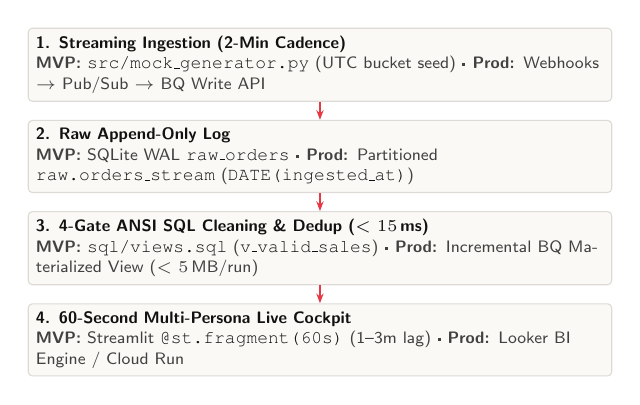
\begin{tikzpicture}[
        box/.style={draw=hairline, fill=cream, rounded corners=1.5pt, text width=2.84in, align=left, inner sep=2.8pt, font=\fontsize{6.1}{7.4}\selectfont},
        arr/.style={-{Stealth[length=3.5pt]}, line width=0.75pt, color=holaflyred}
      ]
        \node[box] (n1) {\textbf{\color{ink}1. Streaming Ingestion (2-Min Cadence)}\\
          {\color{iron}\textbf{MVP:} \code{src/mock\_generator.py} (UTC bucket seed) \textperiodcentered\ \textbf{Prod:} Webhooks $\rightarrow$ Pub/Sub $\rightarrow$ BQ Write API}};

        \node[box, below=0.09in of n1] (n2) {\textbf{\color{ink}2. Raw Append-Only Log}\\
          {\color{iron}\textbf{MVP:} SQLite WAL \code{raw\_orders} \textperiodcentered\ \textbf{Prod:} Partitioned \code{raw.orders\_stream} (\code{DATE(ingested\_at)})}};

        \node[box, below=0.09in of n2] (n3) {\textbf{\color{ink}3. 4-Gate ANSI SQL Cleaning \& Dedup ($<15$\,ms)}\\
          {\color{iron}\textbf{MVP:} \code{sql/views.sql} (\code{v\_valid\_sales}) \textperiodcentered\ \textbf{Prod:} Incremental BQ Materialized View ($<5$\,MB/run)}};

        \node[box, below=0.09in of n3] (n4) {\textbf{\color{ink}4. 60-Second Multi-Persona Live Cockpit}\\
          {\color{iron}\textbf{MVP:} Streamlit \code{@st.fragment(60s)} (1--3m lag) \textperiodcentered\ \textbf{Prod:} Looker BI Engine / Cloud Run}};

        \draw[arr] (n1) -- (n2);
        \draw[arr] (n2) -- (n3);
        \draw[arr] (n3) -- (n4);
      \end{tikzpicture}
    \end{hfcard}
  \end{column}
\end{columns}
\end{frame}

% =============================================================================
% SLIDE 3: WHAT COUNTS AS A SALE (4-GATE DATA QUALITY)
% =============================================================================
\begin{frame}[t]{``What Counts as a Sale?'' --- 4-Gate SQL Standard}{Data Quality \& Auditability}
\vspace{1pt}
\begin{calloutbar}
  {\fontsize{6.5}{8.0}\selectfont \textbf{Formal Business Rule:} A raw order counts as a \textbf{Valid Sale} if and only if it passes all four ordered SQL gates in \code{v\_classified\_orders}. Rejected records remain fully auditable in \code{v\_quarantined\_orders} and the top Telemetry Strip.}
\end{calloutbar}

\vspace{2.5pt}
\renewcommand{\arraystretch}{1.05}
{\fontsize{6.3}{7.6}\selectfont
\begin{tabularx}{\textwidth}{@{}l l >{\raggedright\arraybackslash}X r@{}}
\toprule
\rowcolor{linen}
\textbf{\color{ink}Gate} & \textbf{\color{ink}Quarantine Status} & \textbf{\color{ink}Formal SQL Exclusion / Acceptance Rule} & \textbf{\color{ink}Rate} \\
\midrule
\textbf{Gate 1} & \code{MISSING\_DIMENSION} & Rejects null/blank \code{order\_id}, \code{agent\_name}, or values outside Holafly's 6 markets \& 5 languages. & $\sim 1.0\%$ \\
\rowcolor{purewhite}
\textbf{Gate 2} & \code{TEST\_EMAIL} & Excludes internal QA/staging (\code{@holafly.internal}, \code{@staging.holafly.com}, \code{@testmail.invalid}, \code{qa.*}, \code{test\_*}, \code{loadtest.*}). & $\sim 2.5\%$ \\
\textbf{Gate 3} & \code{INVALID\_AMOUNT} & Requires strictly \textbf{$\text{amount\_usd} > \$0.00$} (filters $\$0$ failed captures \& negative refunds). \textbf{No upper cap:} B2B bundles ($\$640+$) count as valid sales. & $\sim 3.0\%$ \\
\rowcolor{purewhite}
\textbf{Gate 4} & \code{DUPLICATE} & Retains first arrival via \code{ROW\_NUMBER() OVER (PARTITION BY order\_id ORDER BY ingested\_at\_utc ASC, raw\_event\_id ASC) = 1}. & $\sim 4.0\%$ \\
\bottomrule
\end{tabularx}
}

\vspace{3pt}
\begin{columns}[T,onlytextwidth]
  \begin{column}{0.49\textwidth}
    \begin{neutralcard}{Partition Conservation Invariant (T-06)}
      {\fontsize{6.2}{7.7}\selectfont $\text{Raw} \equiv \text{Valid} + \text{Dup} + \text{Invalid Amt} + \text{QA Email} + \text{Missing Dim}$ (\code{Delta = 0}), verified live on Tab 4.}
    \end{neutralcard}
  \end{column}
  \begin{column}{0.49\textwidth}
    \begin{neutralcard}{Why No Arbitrary Upper Cap on Amount?}
      {\fontsize{6.2}{7.7}\selectfont Corporate/group travelers buy 8--15 eSIMs per checkout. A $\$500$ cap would silently drop Holafly's highest-margin B2B sales.}
    \end{neutralcard}
  \end{column}
\end{columns}
\end{frame}

% =============================================================================
% SLIDE 4: LIVE PRODUCT TOUR (SCREENSHOT + 3 PERSONAS)
% =============================================================================
\begin{frame}[t]{Three Operational Personas in One Live Cockpit}{Live Interface \& Shift Decisions}
\vspace{2pt}
\begin{columns}[T,onlytextwidth]
  \begin{column}{0.60\textwidth}
    \begin{tcolorbox}[
      enhanced, colback=purewhite, colframe=hairline, boxrule=0.6pt, arc=1.5pt,
      left=1.5pt, right=1.5pt, top=1.5pt, bottom=1.5pt
    ]
      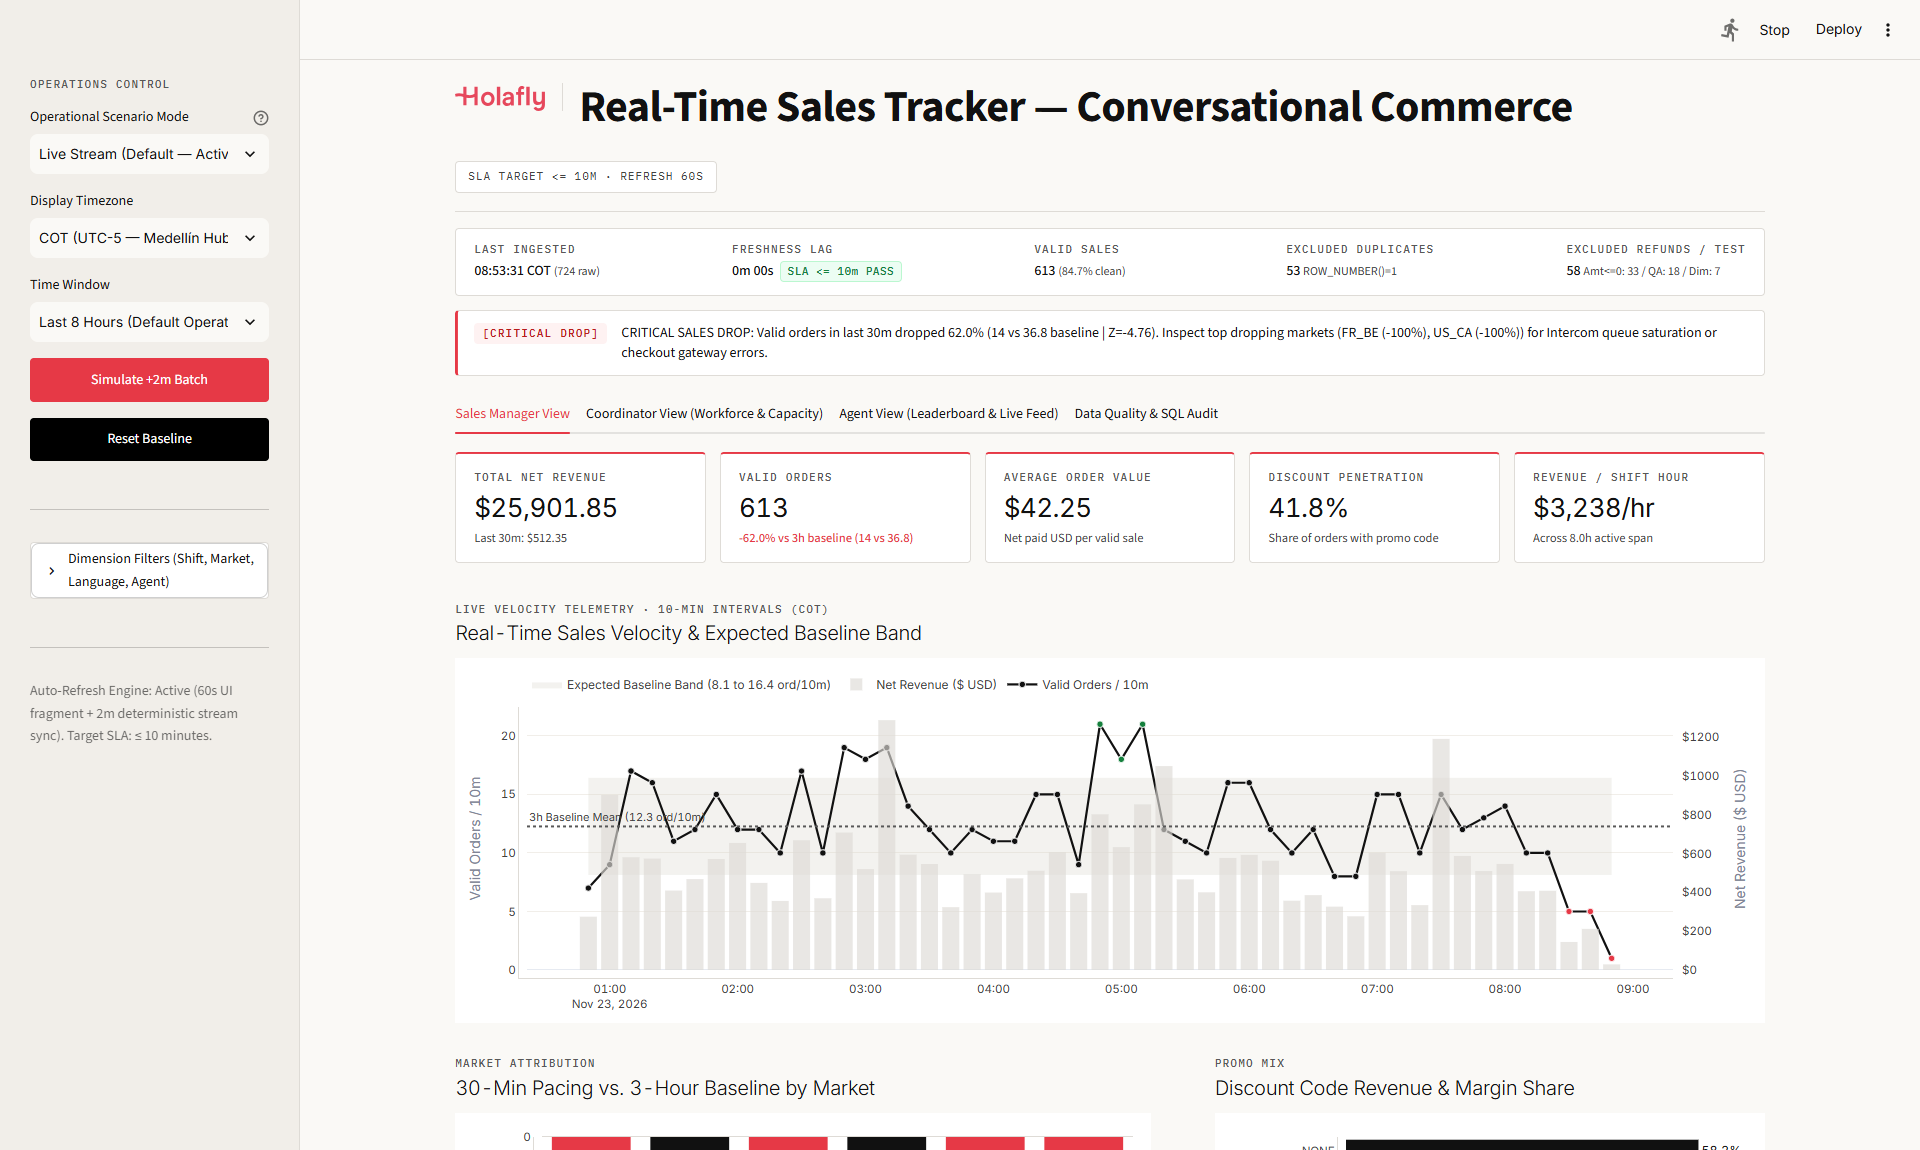
\includegraphics[width=\textwidth]{../static/dashboard_preview.png}
    \end{tcolorbox}
    \vspace{-3pt}
    {\fontsize{6.2}{7.6}\selectfont\color{graphite}Live Playwright capture at 1920$\times$1150: Official Holafly identity, 1-row telemetry strip, restrained alert card, custom non-truncating KPI grid, and organic 10-min velocity band.}
  \end{column}

  \begin{column}{0.38\textwidth}
    \begin{hfcard}[top=2.5pt,bottom=2.5pt,before skip=0pt,after skip=3pt]{1. Sales Manager View}
      {\fontsize{5.9}{7.3}\selectfont Track Net Revenue, Valid Orders, AOV, Discount \%, and Rev/Shift Hr. Catch mid-shift drops or \code{FLASH20} spikes via the baseline band and Market Attribution chart.}
    \end{hfcard}
    \begin{hfcard}[top=2.5pt,bottom=2.5pt,before skip=0pt,after skip=3pt]{2. Coordinator View (WFM)}
      {\fontsize{5.9}{7.3}\selectfont Inspect the \textbf{Market $\times$ Language Matrix} and Action Queue to flex bilingual agents from \code{UNDER-UTILIZED} into \code{OVERLOADED} queues mid-shift.}
    \end{hfcard}
    \begin{hfcard}[top=2.5pt,bottom=2.5pt,before skip=0pt,after skip=0pt]{3. Agent View \& SQL Audit}
      {\fontsize{5.9}{7.3}\selectfont Shift-relative Leaderboard (\code{TOP CLOSER} / \code{ON PACE} / \code{NEEDS COACHING}), latest 25 valid sales ticker, and Tab 4 quarantine log.}
    \end{hfcard}
  \end{column}
\end{columns}
\end{frame}

% =============================================================================
% SLIDE 5: DEFENDING THE RATIOS (I) — WFM CAPACITY & SHIFT PACE
% =============================================================================
\begin{frame}[t]{Defending the Ratios (I): WFM Capacity \& Utilization}{Operational Derivation \& Erlang C Logic}
\vspace{2pt}
\begin{columns}[T,onlytextwidth]
  \begin{column}{0.48\textwidth}
    \begin{hfcard}{Why 3.50 Orders / Agent-Hour Benchmark?}
      {\fontsize{6.6}{8.2}\selectfont Derived from Conversational Commerce funnel math:}
      \vspace{3pt}
      \renewcommand{\arraystretch}{1.16}
      {\fontsize{6.5}{8.0}\selectfont
      \begin{tabularx}{\linewidth}{@{}>{\raggedright\arraybackslash}X r@{}}
        \toprule
        \rowcolor{linen} \textbf{Operational Parameter} & \textbf{MVP Value} \\
        \midrule
        Productive time (17\% shrinkage) & $50\text{ min / hr}$ \\
        Avg eSIM sales handle time (AHT) & $7.5\text{ min / chat}$ \\
        Effective chat concurrency & $2.25\text{ chats}$ \\
        Commercial chats handled & $\sim 15.0\text{ / hr}$ \\
        Chat-to-sale conversion rate & $23.3\%$ \\
        \midrule
        \rowcolor{softgreen} \textbf{Derived Capacity Target} & \textbf{3.50 ord / hr} \\
        \bottomrule
      \end{tabularx}
      }
      \vspace{3pt}
      {\fontsize{6.4}{8.0}\selectfont\color{iron}\textbf{Day-1 Calibration:} Replace \code{3.50} with rolling 28-day empirical median/P60 orders/agent-hr per \code{Market $\times$ Language} from Intercom + BigQuery.}
    \end{hfcard}
  \end{column}

  \begin{column}{0.50\textwidth}
    \begin{neutralcard}{Utilization Bands (Erlang C Saturation Logic)}
      {\fontsize{6.7}{8.5}\selectfont
      \begin{itemize}\setlength\itemsep{2.5pt}
        \item \textbf{\color{holaflyred}OVERLOADED ($\geq 115\%$, $>4.0$ ord/hr):} Why $115\%$ vs.\ $100\%$? Brief 10--15\% bursts are absorbed by concurrency; sustaining $\geq 115\%$ pushes concurrency past 3+ chats, spiking FRT and hurting conversion.
        \item \textbf{\color{forestok}OPTIMAL ($70\%$--$115\%$):} Balanced SLA without idle burn.
        \item \textbf{\color{iron}UNDER-UTILIZED ($< 70\%$, $<2.45$ ord/hr):} $\geq 15$\,min/hr spare capacity safe to flex into overloaded queues.
      \end{itemize}
      }
    \end{neutralcard}
    \vspace{4pt}
    \begin{neutralcard}{Why Shift-Relative Agent Pace ($\pm 15\%$)?}
      {\fontsize{6.7}{8.5}\selectfont Comparing Night/APAC volume to Afternoon Peak introduces timezone bias. Benchmarking agents strictly against \textbf{same-shift peers} isolates closing skill, while $\pm 15\%$ absorbs ticket-size mix ($\$19$ vs.\ $\$69$ eSIMs).}
    \end{neutralcard}
  \end{column}
\end{columns}
\end{frame}

% =============================================================================
% SLIDE 6: DEFENDING THE RATIOS (II) — ANOMALY DETECTION & GUARDRAILS
% =============================================================================
\begin{frame}[t]{Defending the Ratios (II): Anomaly Detection \& Guardrails}{Statistical Noise Control \& Midnight-Safe Shift Math}
\vspace{2pt}
\begin{columns}[T,onlytextwidth]
  \begin{column}{0.51\textwidth}
    \begin{hfcard}{Why 30-Min Window vs. 180-Min Baseline?}
      {\fontsize{6.7}{8.5}\selectfont Order arrivals follow a Poisson process ($\sigma \approx \sqrt{\mu}$):
      \begin{itemize}\setlength\itemsep{2.5pt}
        \item \textbf{10-Min Window ($\mu \approx 12$):} Random noise is $\pm\sqrt{12}/12 = \mathbf{\pm 29\%}$---too noisy for reliable alerting.
        \item \textbf{30-Min Window ($\mu \approx 36$):} Relative noise falls to $\mathbf{\pm 16.7\%}$, while catching incidents \textbf{8--10$\times$ faster than Looker's 3--5h lag}.
        \item \textbf{Dual Trigger (\% Delta + Z-Score):}
          \begin{itemize}\setlength\itemsep{1.5pt}
            \item \textbf{\color{amberwarn}WARNING ($\leq -20\%$ or $Z \leq -1.8$):} Early FRT/queue watch.
            \item \textbf{\color{holaflyred}CRITICAL DROP ($\leq -35\%$ or $Z \leq -2.5$):} $<1\%$ chance by luck $\rightarrow$ escalate checkout/Intercom check.
            \item \textbf{\color{forestok}SURGE ($\geq +35\%$ or $Z \geq +2.5$):} Flex stand-by agents.
          \end{itemize}
      \end{itemize}
      }
    \end{hfcard}
  \end{column}

  \begin{column}{0.47\textwidth}
    \begin{neutralcard}[top=3pt,bottom=3pt]{False-Alarm Guard ($\mu_{\text{base}} \geq 10$ / 30m)}
      {\fontsize{6.2}{7.7}\selectfont Filtering down to one agent ($\mu=2$) closing 1 order is mathematically ``$-50\%$'' despite normal variance. Suppressing alerts below $\mu_{\text{base}}=10$ eliminates alert fatigue.}
    \end{neutralcard}
    \vspace{2.5pt}
    \begin{neutralcard}[top=3pt,bottom=3pt]{Midnight-Safe Math (\code{SHIFT\_3\_NIGHT})}
      {\fontsize{6.2}{7.7}\selectfont All elapsed-hour, rolling 30m/180m, and \textit{Current Active Shift Only} filters run strictly on \textbf{full UTC timestamps}, unifying \code{22:00} prev-day through \code{05:59 COT} without splitting at midnight.}
    \end{neutralcard}
    \vspace{2.5pt}
    \begin{calloutbar}[ink]
      {\fontsize{6.1}{7.6}\selectfont \textbf{Day-1 Upgrade:} Swap trailing 3h baseline for a \textbf{Same-Hour, Same-Weekday (4-week rolling median/MAD)} baseline from BigQuery so predictable morning ramps never trigger false surges.}
    \end{calloutbar}
  \end{column}
\end{columns}
\end{frame}

% =============================================================================
% SLIDE 7: AI WORKFLOW & 15-TEST QUANTITATIVE VALIDATION
% =============================================================================
\begin{frame}[t]{AI-First Workflow \& Quantitative Validation Protocol}{Human-in-the-Loop Governance \& Caught Edge Cases}
\vspace{2pt}
\begin{columns}[T,onlytextwidth]
  \begin{column}{0.46\textwidth}
    \begin{hfcard}{Spec-First AI Engineering Discipline}
      {\fontsize{6.8}{8.7}\selectfont
      \begin{itemize}\setlength\itemsep{3.5pt}
        \item \textbf{Human Analyst Ownership:} Locked architecture, WFM funnel ratios, 4-gate SQL rules, and Holafly editorial design inside \code{spec.md} \textit{before} generating code.
        \item \textbf{AI Acceleration (Antigravity IDE):} Accelerated Streamlit scaffolding, Plotly formatting, LaTeX typesetting, and test suite boilerplate.
        \item \textbf{Zero Blind Trust:} Every SQL gate, KPI formula, and UI render is guarded by \textbf{15 automated \code{pytest} assertions} + live Playwright browser verification.
      \end{itemize}
      }
    \end{hfcard}
  \end{column}

  \begin{column}{0.52\textwidth}
    \begin{neutralcard}{4 Real Bugs Caught \& Fixed During Validation}
      {\fontsize{6.6}{8.4}\selectfont
      \begin{enumerate}\setlength\itemsep{3pt}
        \item \textbf{Off-Shift Coverage Gap:} An 8h-only backfill left one shift empty depending on clock hour $\rightarrow$ upgraded DB storage to a rolling 24h 3-shift cycle while keeping 8h default UI focus (\code{T-01}).
        \item \textbf{Artificial Flat Baseline:} Fixed cycling caused a flat 12-order line $\rightarrow$ upgraded to diurnal wave + Knuth Poisson variance (\code{T-14}).
        \item \textbf{Markdown HTML Indentation Bug:} 4-space indentation caused raw \code{<div class="kpi-card">} leakage $\rightarrow$ flattened all HTML emitters + added DOM regression guard (\code{T-15}).
        \item \textbf{Arbitrary \$500 Cap Removed:} Removed upper cap so legitimate high-value B2B bundles ($\$640+$) count as valid sales (\code{T-03}).
      \end{enumerate}
      }
    \end{neutralcard}
  \end{column}
\end{columns}
\end{frame}

% =============================================================================
% SLIDE 8: DAY-1 PRODUCTION ROADMAP AT HOLAFLY
% =============================================================================
\begin{frame}[t]{Day-1 Production Roadmap at Holafly}{From Lean MVP to Production Real-Time Operations}
\vspace{2pt}
\begin{columns}[T,onlytextwidth]
  \begin{column}{0.32\textwidth}
    \begin{hfcard}{Phase 1 \textperiodcentered\ Week 1}
      \textbf{\color{ink}\fontsize{7.5}{9}\selectfont Live BigQuery Streaming}\\[2pt]
      {\fontsize{6.6}{8.4}\selectfont
      \begin{itemize}\setlength\itemsep{2.5pt}
        \item Connect Checkout \& Intercom webhooks via Pub/Sub $\rightarrow$ \textbf{BigQuery Storage Write API}.
        \item Deploy 4-gate SQL as an \textbf{Incremental Materialized View} scanning trailing 24h ($<5$\,MB/run).
        \item Validate \code{Lag <= 2m} vs.\ legacy Looker.
      \end{itemize}
      }
    \end{hfcard}
  \end{column}

  \begin{column}{0.32\textwidth}
    \begin{hfcard}{Phase 2 \textperiodcentered\ Week 2}
      \textbf{\color{ink}\fontsize{7.5}{9}\selectfont Empirical Ratio Calibration}\\[2pt]
      {\fontsize{6.6}{8.4}\selectfont
      \begin{itemize}\setlength\itemsep{2.5pt}
        \item Replace \code{3.50} with rolling 28-day empirical \code{Orders/Agent-Hr} per \code{Market $\times$ Language}.
        \item Upgrade anomaly baseline to \textbf{Same-Hour, Same-Weekday 4-week median/MAD}.
        \item Join live Intercom FRT \& chat concurrency.
      \end{itemize}
      }
    \end{hfcard}
  \end{column}

  \begin{column}{0.32\textwidth}
    \begin{hfcard}{Phase 3 \textperiodcentered\ Weeks 3--4}
      \textbf{\color{ink}\fontsize{7.5}{9}\selectfont Automated WFM Action Loop}\\[2pt]
      {\fontsize{6.6}{8.4}\selectfont
      \begin{itemize}\setlength\itemsep{2.5pt}
        \item Host cockpit on \textbf{Google Cloud Run (\code{min-instances=1})}---zero cold starts.
        \item Trigger Slack/WhatsApp alerts on \code{CRITICAL DROP} \& \code{OVERLOADED} queues.
        \item Add Erlang C staggered shift optimizer for AMER/EMEA/APAC handoffs.
      \end{itemize}
      }
    \end{hfcard}
  \end{column}
\end{columns}

\vspace{5pt}
\begin{calloutbar}[holaflyred]
  {\fontsize{6.7}{8.4}\selectfont \textbf{\color{ink}Closing Takeaway:} \color{iron}Built lean to eliminate Holafly's 3--5 hour visibility blind spot today---and engineered cleanly to plug directly into BigQuery, Intercom, and WFM capacity planning on Day 1.\\
  \color{graphite}\textbf{Live Demo:} \href{https://holafly-realtime-sales-tracker.streamlit.app/}{\color{holaflyred}\code{holafly-realtime-sales-tracker.streamlit.app}} \quad|\quad Gabriel Andr\'es Salazar Espinosa \textperiodcentered\ \code{gabrielandressalazarespinosa@gmail.com}}
\end{calloutbar}
\end{frame}

\end{document}
